The results separated two questions: which content cue drove a response, and how that response changed when the predictor was refitted. Generated tasks tested cue discrimination, and Fidel-TS provided a positive natural-data example. Table~\ref{tab:capability_overview} summarizes capability and coverage evidence for the irregular-data cases.

\subsection{Selective content edits discriminate direction from source}

Selective edits distinguished direction from source, despite a whole-permutation response to both cues. Direction signs and arbitrary Cedar/Maple source cues were generated independently in twenty irregular worlds per target mechanism. Targets depended on direction, source or available-note count alone. Each edit retained the alternative cue within the finite test vocabulary (Table~\ref{tab:construct_examples}).

\begin{table}[htbp]
\centering\small
\caption{One paired example from the frozen construct configuration's test and paraphrase templates. Each selective edit changes one stipulated cue while retaining the other; the paraphrase retains both. Targets and the event process remain fixed.}
\label{tab:construct_examples}
\begin{tabular}{@{}>{\raggedright\arraybackslash}p{0.18\linewidth}>{\raggedright\arraybackslash}p{0.78\linewidth}@{}}
\toprule
Condition & Text at the same event slot\\
\midrule
Aligned & We predict that demand will increase in the upcoming interval. Bulletin source: Cedar.\\
Direction flip & We predict that demand will decrease in the upcoming interval. Bulletin source: Cedar.\\
Source flip & We predict that demand will increase in the upcoming interval. Bulletin source: Maple.\\
Paraphrase & An increase in demand is forecast for the interval ahead. Bulletin source: Cedar.\\
\bottomrule
\end{tabular}
\end{table}


Whole permutation, implemented as nonzero cyclic shifts within available histories, detected content-position reliance in 20/20 worlds for both content targets. All these worlds met the post-selection nominal validation screen for incremental content benefit. On the source-only task, whole permutation increased mean MSE by 0.770870 (across-world 95\% interval [0.758012,0.783728]). Direction flip gave $-0.000228$ [$-0.000640$,0.000185], whereas source flip gave 2.872553 [2.840252,2.904853]. The direction-only task showed the complementary pattern: direction flip gave 2.698159 [2.667529,2.728789], and source flip gave $-0.000071$ [$-0.001688$,0.001546]. Selective edits thus identified which stipulated cue drove the dependence detected by whole permutation.

Paraphrasing preserved the generated cues but changed forecasting error. Direction and source probes recovered cue signs in all sixteen test sentences and sixteen paraphrases. Mean MSE fell by 0.030132 on direction targets and 0.005214 on source targets. One direction world and three source worlds nevertheless showed significant degradation. Recoverable cues therefore did not make the predictor invariant to wording.

For timing-only targets, whole permutation gave $-0.000195$ [$-0.000681$,0.000290] and one ungated rejection. No world met the incremental content-benefit screen against the numerical/timing comparator. Its retained event timing/counts defined the process-only boundary for the content test. Complete-stream MMU was not evaluated because no numerical-only comparator was fitted. Table~\ref{tab:construct_full} reports all fifteen predefined outcomes.

\begin{figure}[!htbp]
\centering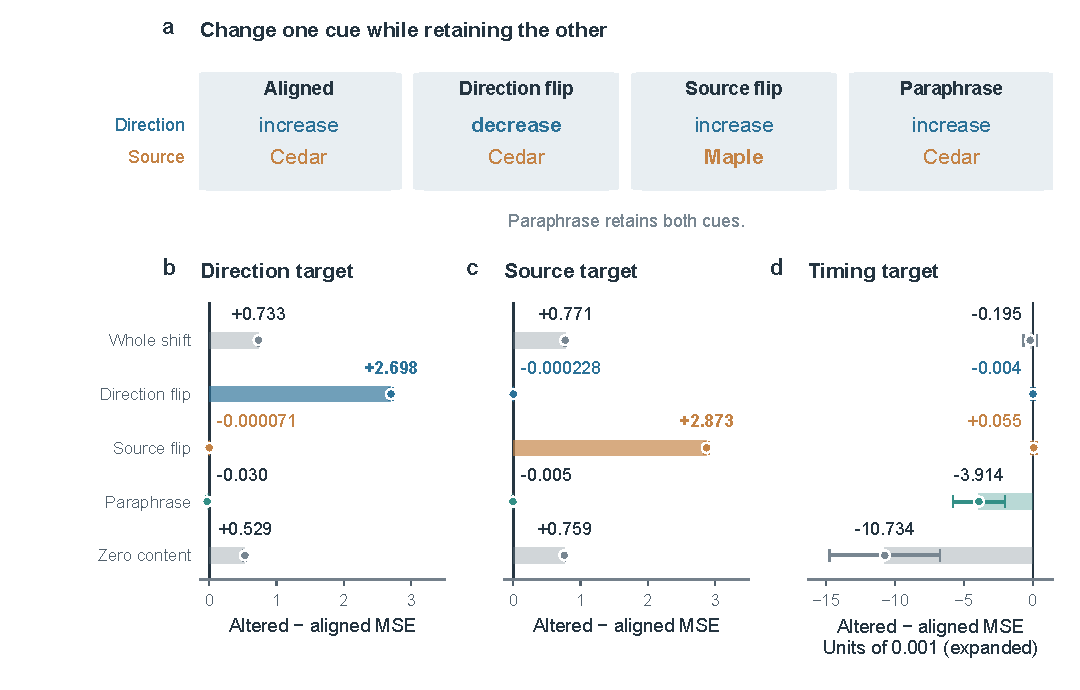
\includegraphics[width=\textwidth]{fig7_construct}
\caption{Selective content edits discriminate the stipulated target cue. (a) Abbreviated direction/source examples show which cue changes; paraphrases change wording while preserving both cues. (b--d) All fifteen fixed-predictor altered-minus-aligned MSE effects for direction, source and timing targets. Points show means and whiskers the saved 95\% $t$ intervals across twenty generated worlds, conditional on shared empirical clocks. Direction and source panels share their scale; the timing axis is expanded in units of 0.001. This contrast concerns the stated cues within the finite generated vocabulary. Table~\ref{tab:construct_full} retains rejection fractions and adverse paraphrase outcomes.}
\label{fig:construct}
\end{figure}


\subsection{Fixed-model reliance and condition-retrained value differ on photovoltaic data}

Refitting reduced the alignment effect in the independent timestamp-restricted Fidel-TS ridge experiment. All nine plants contributed 3,285 daily test windows and 78,840 hourly targets. Numerical-only MSE was 0.191132, compared with 0.181786 for aligned published weather embeddings, giving 4.89\% complete-stream utility. A nonzero cyclic shift of the shared within-split report sequence raised fixed-predictor MSE to 0.226247, giving 19.65\% SAG. Condition-retrained MSE was 0.199692, or 8.97\% SAG, with the same numerical histories and splits. Saved validation comparisons provide descriptive context for overall predictive capability and complete-stream utility (Table~\ref{tab:capability_overview}).

Fixed-shift minus aligned MSE was positive at every plant (0.030509--0.055470); the pooled effect stayed positive across twenty additional maps (Table~\ref{tab:maps}). Plant differences and repeated daily windows share weather context, so they describe heterogeneity without independent replication. The zero-input contrast gave MSE 0.482045 for the same predictor. Median replacement weather-embedding cosine fell from 0.98272 to 0.05801 after training-centroid centering. High raw embedding similarity thus coexisted with a measurable alignment response.

\begin{figure}[!htbp]
\centering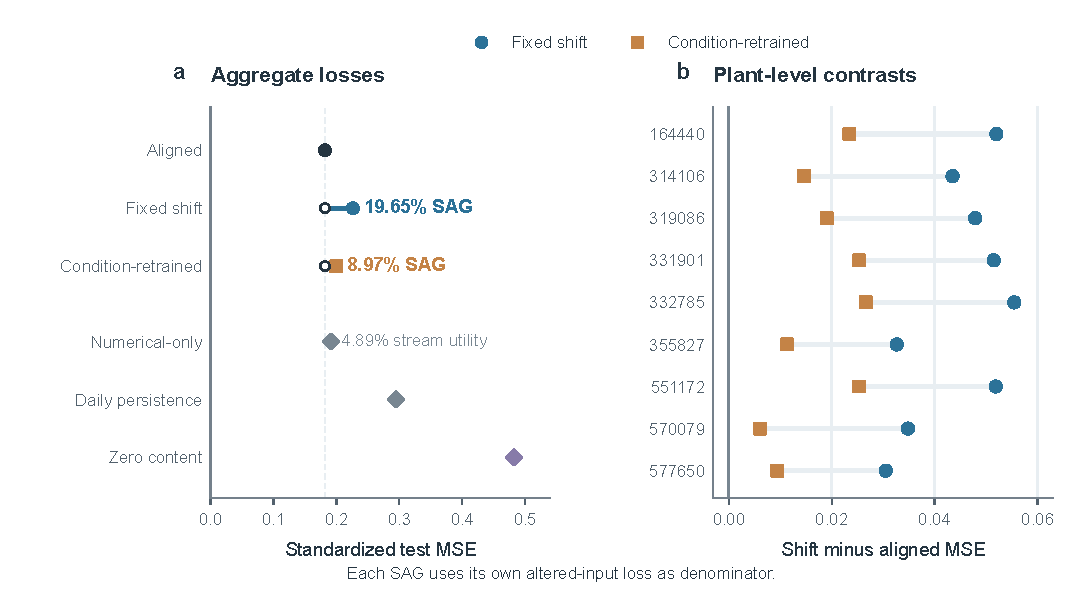
\includegraphics[width=\textwidth]{fig5_fidel}
\caption{Fixed-model reliance and condition-retrained value on the photovoltaic task. (a) Aggregate losses compare the saved input/model conditions. (b) Paired effects connect fixed-shift and retrained-shift contrasts for nine plants. Gains use the corresponding altered-condition MSE as denominator. Plant differences describe heterogeneity under shared weather context, rather than independent-map uncertainty. All 3,285 test windows are retained. Aligned inputs use reports timestamped no later than the cutoff; offline shifts can assign later-dated donors. Issuance and arrival metadata are unavailable.}
\label{fig:fidel}
\end{figure}

\begin{table}[!ht]
\centering\footnotesize
\setlength{\tabcolsep}{4pt}
\caption{Capability evidence and interpretation by batch. Real-data validation comparisons are descriptive; no formal screen was applied. Persistence addresses overall prediction, while a numerical/event comparator addresses incremental content benefit. Fidel's numerical-only comparison measures complete-stream utility. Repeated-map draws retain the aligned model and use the ridge rows' circular-shift families.}
\label{tab:capability_overview}
\begin{tabular}{@{}>{\raggedright\arraybackslash}p{0.20\textwidth}>{\raggedright\arraybackslash}p{0.31\textwidth}>{\raggedright\arraybackslash}p{0.17\textwidth}>{\raggedright\arraybackslash}p{0.25\textwidth}@{}}
\toprule
Evaluation and intervention & Validation evidence and screening status & Achieved intervention & Test evidence\\
\midrule
Historical fixed neural models; restricted random permutation and full derangement & Archived persistence, time-only and aligned validation losses (Table~\ref{tab:historical_validation}). Formal screen: \emph{Not assessed}; 4/45 selections at epoch zero. & Derangement: 56.25\% on CESNET; 100\% elsewhere. & Very small fixed effects; interpretation remains conditional on these checkpoints and maps.\\
Linear known-signal calibration; nonzero within-history rotation & Fixed fitting settings. Incremental-benefit screen: 0/20 null worlds; 20/20 at each nonzero strength, for both representations. & 97.27\% of source positions; 48.52\% of direction values. & Known signal detected in 20/20 worlds per nonzero cell; unscreened null detections 3/20 and 2/20.\\
Construct ridge models; nonzero within-history rotation and cue edits & Same-sample ridge selection and post-selection nominal screen: direction/source 20/20; timing 0/20. & Empty and singleton histories retained; alternative cue preserved in each targeted edit. & Whole-content effects occur for both cues; targeted flips distinguish the generated cue used.\\
EPA-Air ridge; nonzero entity/split circular shift & Persistence validation MSE 1.075034; aligned 0.901160--0.968275. Only FinBERT improves the numerical/timing mean. Formal screen: \emph{Not assessed}. & All selected representations change; latest-four-note summary. & All models lose to test persistence; fixed pooled effects are negative.\\
FNSPID ridge; nonzero entity/split circular shift & Persistence validation MSE 0.648214; aligned 0.673852--0.680205. No overall mean improvement. Formal screen: \emph{Not assessed}. & All selected representations change; latest-four-note summary. & Fixed pooled effects are negative; later test gains do not qualify validation capability.\\
Fidel ridge; nonzero shift of shared split report sequence & Validation numerical 0.221023; aligned 0.208860; persistence 0.350711. Descriptive stream utility 5.50\%. Formal screen: \emph{Not assessed}. & All recipient weather vectors change; one common map across nine plants. & Fixed $\Delta$ MSE +0.044461; retrained +0.017906. The two effects answer different questions.\\
\bottomrule
\end{tabular}
\end{table}

The batches resolve different questions: EPA-Air separates validation improvement from later transfer; FNSPID separates incremental content benefit from overall prediction; Fidel demonstrates complete-stream utility in a regular task. Historical validation losses contextualize fixed-checkpoint effects without adding a screening decision. Full losses and selected epochs appear in Tables~\ref{tab:historical_validation} and~\ref{tab:ridge_capability_details}.


\subsection{Known-signal calibration reveals detection sensitivity and null errors}

Oracle-direction and templated MiniLM predictors detected known signal in 20/20 worlds at each nonzero strength, $\gamma=0.25,0.5,1$. The Wilson 95\% interval for this rate was 83.9--100\%. MiniLM's mean fixed-shift MSE differences were 0.046804, 0.186640 and 0.745574, in strength order. Corresponding across-world 95\% intervals were [0.045030,0.048578], [0.182506,0.190775] and [0.734231,0.756917]. Its held-out direction probe recovered all eight test phrasings, showing recoverability within this controlled vocabulary.

Before screening, null rejection occurred in 3/20 oracle worlds (15\%; Wilson interval 5.2--36.0\%) and 2/20 MiniLM worlds (10\%; 2.8--30.1\%). The descriptive validation screen for incremental content benefit admitted no null world and all tested nonzero worlds. The joint screen-and-detection fraction for null worlds was therefore 0/20, with an upper Wilson bound of 16.1\%. This generator-specific result does not establish a general 5\% error-control guarantee.

Nonzero cyclic shifts within available histories changed 97.27\% of source positions but 48.52\% of direction values. Of test queries, 18.40\% had no available note and 10.41\% had one; all remained in the analysis. Repeated directions preserved some content despite changes in source position. These results describe the evaluated linear pipeline on generated propositions and targets under eight empirical timing templates.

\begin{figure}[!htbp]
\centering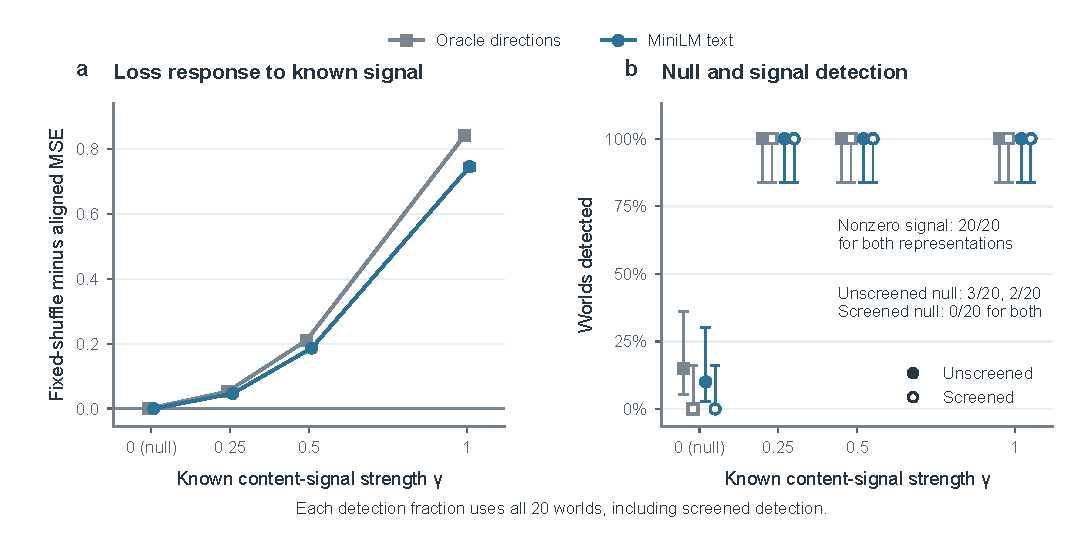
\includegraphics[width=\textwidth]{fig3_calibration}
\caption{Signal-strength calibration under irregular empirical timing templates. (a) Mean fixed-shift minus aligned MSE with saved 95\% $t$ intervals over twenty generated worlds. (b) Unscreened and screened detection fractions with Wilson 95\% intervals. Filled markers show unscreened detection and open markers screened detection; screened detection is the joint screen-and-detection fraction over all twenty worlds. Each within-world test pairs 128 generated entities after averaging three optimizer seeds. Strengths reuse inputs within a world.}
\label{fig:calibration}
\end{figure}

\subsection{Small historical reassignment effects coexist with zero-content sensitivity}

Across fifteen historical dataset/mechanism cells, the largest absolute mean full-derangement change relative to aligned MSE was 0.005868\%, on CESNET cross-attention. Paired block-length 2, 4 and 8 intervals all spanned zero. Four aligned checkpoints selected epoch zero: all three CESNET cross-attention seeds and FNSPID cross-attention seed 53. Tables~\ref{tab:capability_overview} and \ref{tab:fixed_population} provide archived validation context and retained populations; all 45 checkpoints remain formally unassessed for capability screening.

For RecAvg, control-denominator CBTG was 5.119\%, 10.476\%, 10.426\%, 22.726\% and 12.411\% on ClusterTrace, CESNET, EPA-Air, FNSPID and RepoHealth, respectively. The training-content centroid changed MSE by less than 0.005\% of aligned MSE for the same mechanism. Mean zero-content sensitivity thus exceeded sensitivity to content-position pairing. Because zero vectors change representation support as well as information, their loss increase alone does not identify aligned semantic use.

CESNET's nominal doses differed from their achieved interventions. Neither the 25\% nor 50\% dose changed a source position because the per-entity subsets were too small to derange. The 75\% dose changed 12.5\% of all positions, and the full dose changed 56.25\%. These effects concern the selected checkpoints and realized interventions; intervals spanning zero do not establish practical equivalence.

\begin{figure}[!htbp]
\centering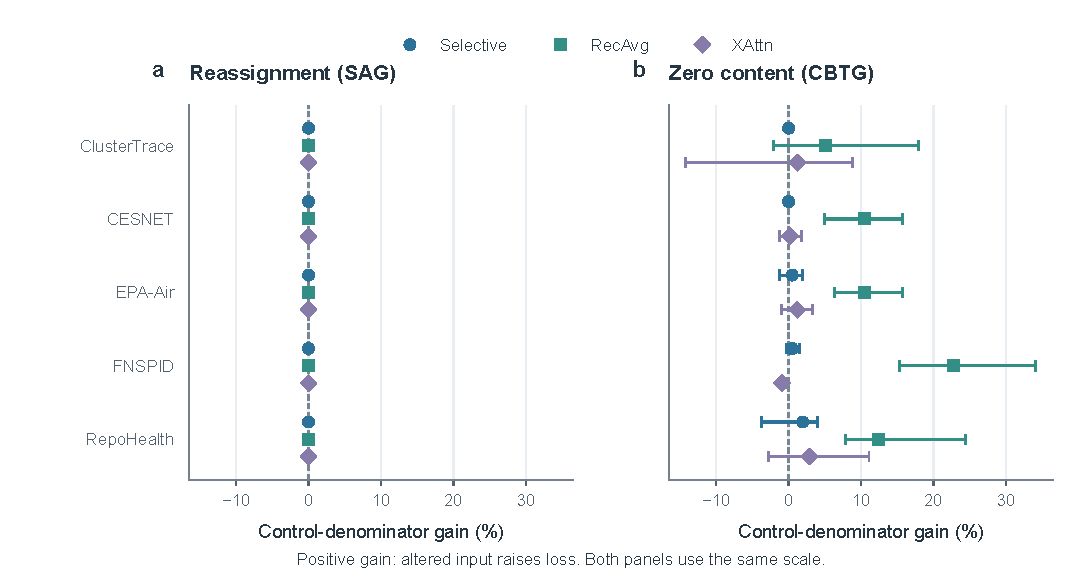
\includegraphics[width=\textwidth]{fig4_fixed_model}
\caption{Same-checkpoint reassignment and zero-content effects across three mechanisms and five datasets. Points show control-denominator $100(L_{\rm altered}-L_{\rm aligned})/L_{\rm altered}$: fixed SAG for full derangement and CBTG for zero input. Bars are the saved paired entity/window-block bootstrap 95\% intervals with block length two; each cell averages three aligned checkpoints. Both panels use the same percentage scale. All fifteen derangement intervals span zero. Full effect records and retained populations appear in Tables~\ref{tab:fixed_full} and~\ref{tab:fixed_population}.}
\label{fig:fixed}
\end{figure}

\subsection{Representation geometry and forecasting transfer require separate checks}

\begin{figure}[!htbp]
\centering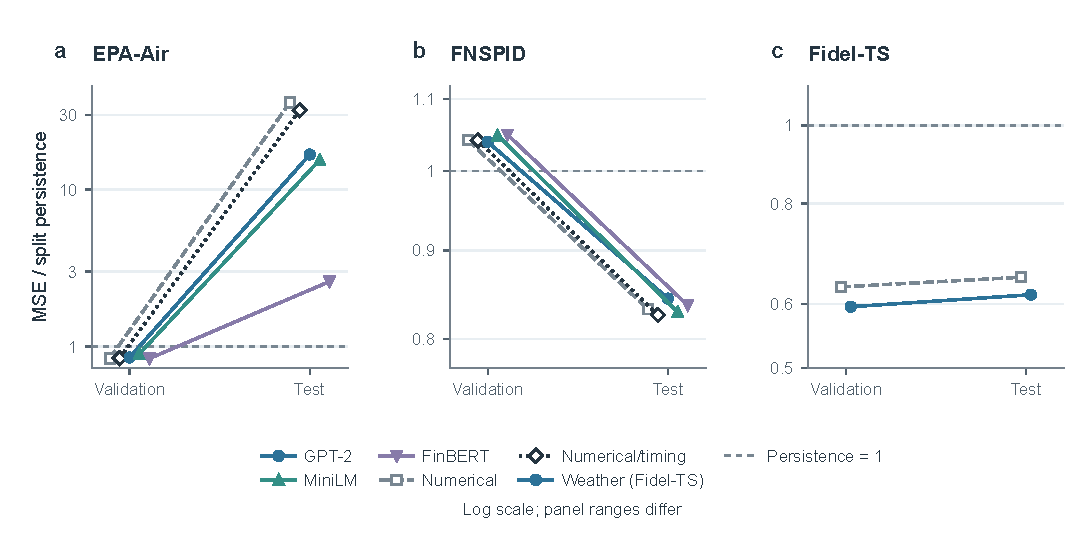
\includegraphics[width=\textwidth]{fig8_transfer}
\caption{Validation comparisons and later test transfer of independent ridge models. Pooled observed-scalar MSE is divided by persistence MSE from the same split; one is the baseline and lower is better. The vertical axis is logarithmic. EPA-Air and FNSPID include numerical, numerical/timing and three aligned text configurations; Fidel-TS includes numerical-only and aligned weather configurations relative to seasonal persistence. Each line connects one validation-selected state across splits. Ratios are descriptive transformations of saved means. Exact losses and penalties appear in Table~\ref{tab:ridge_capability_details}; perturbation contrasts appear in Table~\ref{tab:representations}.}
\label{fig:transfer}
\end{figure}

Validation comparisons and later test transfer are shown in Figure~\ref{fig:transfer}; fixed-model and retrained contrasts are reported in Table~\ref{tab:representations}.


A training-only probe on twelve financial direction sentences allowed MiniLM and FinBERT to classify all twelve differently phrased held-out sentences correctly. The probed direction is therefore recoverable within this vocabulary; forecasting performance requires separate evidence.

Replacement geometry also depends on a shared representation component. On FNSPID, GPT-2's median replacement cosine falls from 0.998964 to 0.188214 after subtracting the training centroid; MiniLM's falls from 0.454059 to 0.142177. On EPA-Air, FinBERT's median falls from 0.768842 to $-0.013962$. Raw cosine can thus be dominated by a shared direction and does not determine whether a task-relevant proposition changed.

On EPA-Air, all three content models improve the validation mean over persistence (1.075034). Only FinBERT improves over numerical/timing ridge (0.901160 versus 0.906853, a descriptive 0.63\% benefit). Every model loses to test persistence (0.751407), including numerical-only and numerical/timing ridge with MSEs of 27.056535 and 24.127104. Negative fixed-shuffle differences therefore accompany poor test-period transfer.

On FNSPID, persistence validation MSE is 0.648214, below numerical ridge (0.675381), numerical/timing ridge (0.675222) and all three content models (0.673852, 0.679578 and 0.680205). GPT-2's 0.20\% mean improvement over numerical/timing ridge thus provides no overall capability advantage. Later gains over test persistence (0.320936) cannot retrospectively qualify validation capability. No formal paired validation screen was applied to these representation comparisons.

Aggregation can reverse the effect's direction. For EPA-Air FinBERT, fixed shuffle reduces scalar-pooled MSE from 1.950746 to 1.945247 but increases entity-macro MSE from 2.388571 to 2.398929. Three of eight entities have a positive alignment point effect. FNSPID has 4/10 such entities for GPT-2, 2/10 for MiniLM and 4/10 for FinBERT. The pooled endpoint therefore need not represent a common entity-level direction.


\subsection{Repeated maps distinguish stable responses from map-sensitive effects}

Fidel's fixed-model response stayed positive under all twenty additional within-split nonzero cyclic shifts. Mean $\Delta$ MSE was 0.047600, the empirical 2.5th--97.5th percentile range was [0.032916,0.064487], and mean map-wise control-denominator SAG was 20.65\%. Positive-map counts for GPT-2, MiniLM and FinBERT were 0/20, 3/20 and 3/20 on FNSPID, and 2/20, 6/20 and 8/20 on EPA-Air. EPA-Air's effect direction thus depended on the map with model states and targets held fixed; Table~\ref{tab:maps} summarizes all seven cells.

Figure~\ref{fig:map_sensitivity} shows intervention-map sensitivity at the selected aligned states, separately from variation across entities or fitted models. Although aligned histories remained timestamp-restricted, offline shifts could assign later-dated donors; Supplementary Section~\ref{sec:map_conditioning} reports their timing fractions and denominators.

\begin{figure}[!htbp]
\centering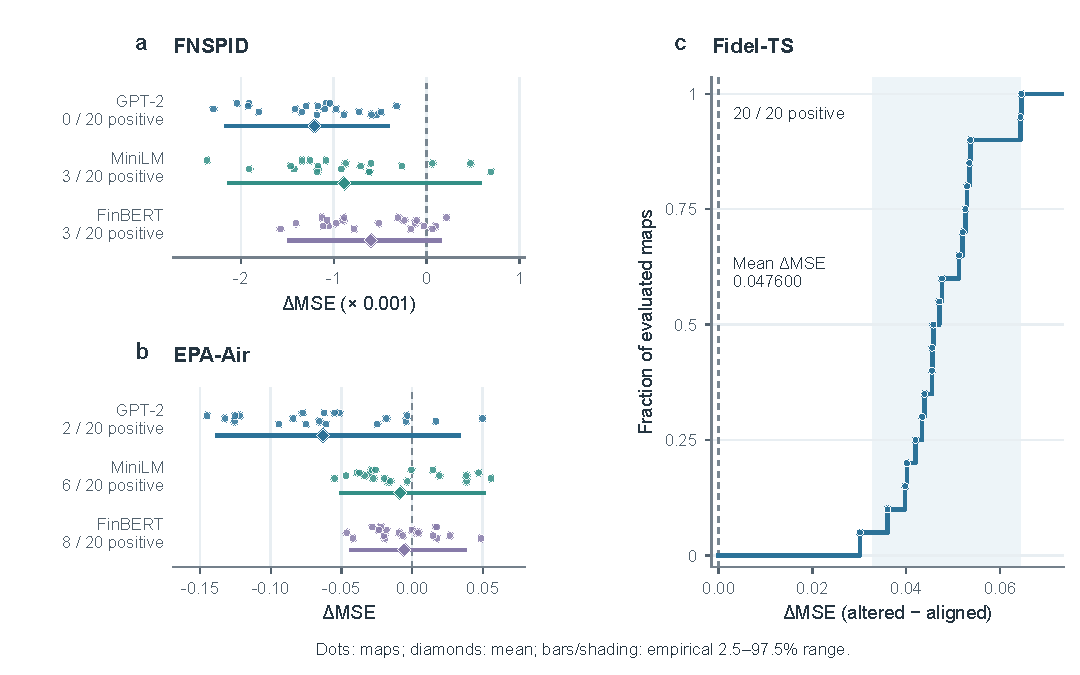
\includegraphics[width=\textwidth]{fig9_map_sensitivity}
\caption{Variation of fixed-model loss effects across the saved nonzero cyclic-shift maps. All 140 altered-minus-aligned MSE effects are retained: three encoder cells on FNSPID, three on EPA-Air and one shared-weather cell on Fidel. Each cell uses twenty maps of the same selected aligned state. (a,b) Encoder-specific effects are shown as strips. (c) Fidel effects are ordered by their empirical cumulative fraction. Zero separates greater altered-input loss from improvement. Bars and shading show saved 2.5th--97.5th percentiles over twenty maps, rather than sampling confidence intervals. Dataset-specific scales reflect different effect magnitudes. The numeric summaries appear in Table~\ref{tab:maps}.}
\label{fig:map_sensitivity}
\end{figure}


